% !TeX root = ../D4.3a_User_Manual.tex

\section{Modelio and SysML}
\label{sec:SysML}
The INTO-CPS tool chain supports a model-based approach to the development and validation of CPS.
%
The Modelio tool and its SysML/INTO-CPS profile extension provide the diagramming starting point.
%
This section describes the Modelio extension that provides INTO-CPS-specific modelling functionality to the SysML modelling approach.

The INTO-CPS extension module is based on the Modelio SysML extension module, and extends it in order to fulfill INTO-CPS modelling requirements and needs.
%
\autoref{figure:into-cps-example} shows an example of a simple INTO-CPS Architecture Structure Diagram under Modelio.
%
%
%
\begin{figure}[hpt!]
\centering
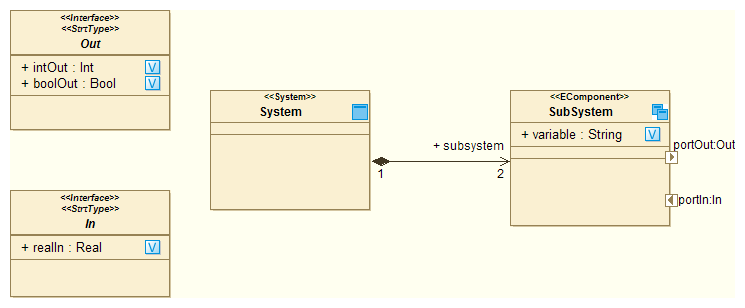
\includegraphics[width=\textwidth]{./figures/modelio-intocps-extension.png}
\caption{Example INTO-CPS multi-model.}
\label{figure:into-cps-example}
\end{figure}
%
%
%
This diagram shows a \textit{System}, named ``System''\footnote{An abstract description of an INTO-CPS multi-model.},  composed of two \textit{EComponent}s of kind \textit{Subsystem}, named ``SubSystem''\footnote{Abstract descriptions of INTO-CPS constituent models.}. These \emph{Subsystem}s have an internal \textit{Variable} called ``variable'' of type \textit{String} and expose two \textit{FlowPort}s named ``portIn'' and ``portOut''. The type of data going through these ports is respectively defined by types \emph{In} and \emph{Out} of kind \textit{StrtType}.
%
More details on the SysML/INTO-CPS profile can be found in Deliverable D2.3a \cite{INTOCPSD2.3a}.

\autoref{figure:sysml-general-aspect} illustrates the main graphical interface after Modelio and the INTO-CPS extension have been installed.
%
%
\begin{figure}[hpt!]
\centering
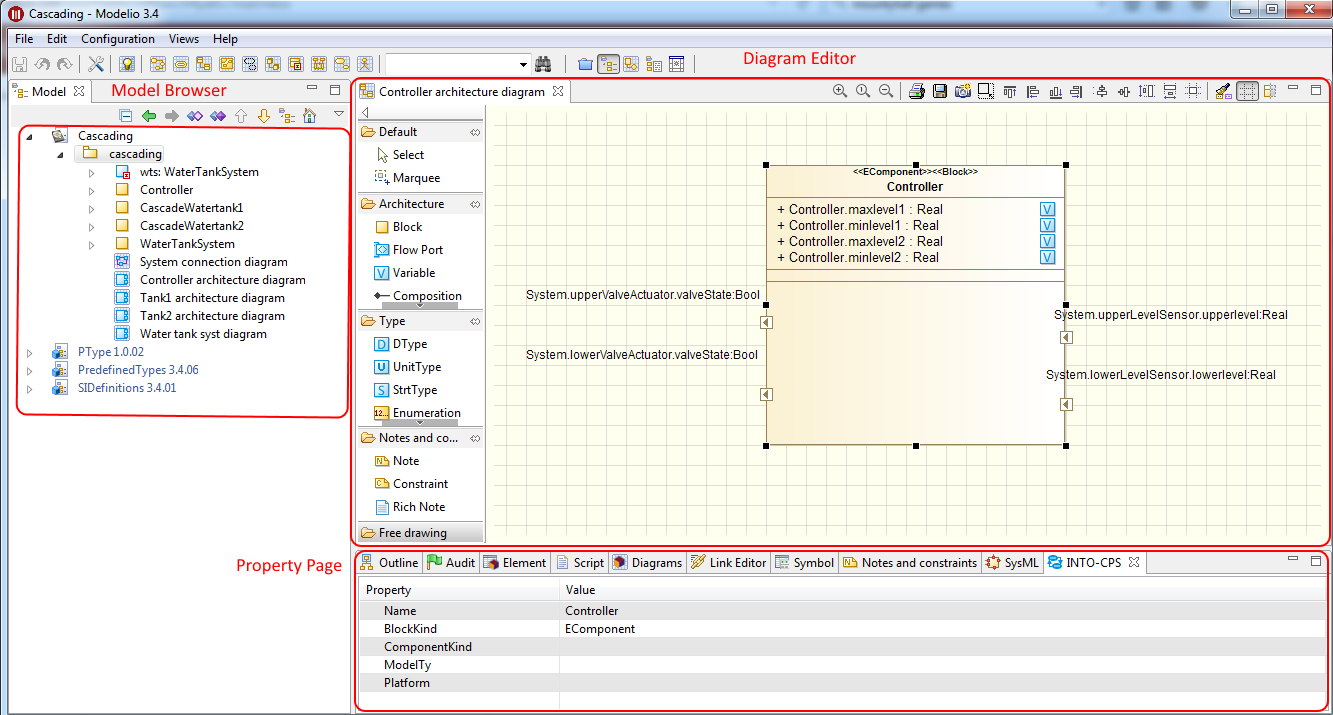
\includegraphics[width=\textwidth]{./figures/sysml-general-aspect.png}
\caption{Modelio for INTO-CPS.}
\label{figure:sysml-general-aspect}
\end{figure}
%
%
Of all the panes, the following three are most useful in the INTO-CPS context.
%
%
%
\begin{enumerate}
\item The Modelio model browser, which lists all the elements of your model in tree form.
\item The diagram editor, which allows you to create INTO-CPS design architectures and connection diagrams.
\item The INTO-CPS property page, in which values for properties of INTO-CPS subsystems are specified.
\end{enumerate}
%
%
%
\subsection{Creating a New Project}
In the INTO-CPS Modelling workflow described in Deliverable D3.3a \cite{INTOCPSD3.3a}, the first step will be to create, as depicted in \autoref{figure:modelio-project-creation}, a Modelio project:

%
\begin{figure}[hpt!]
\centering
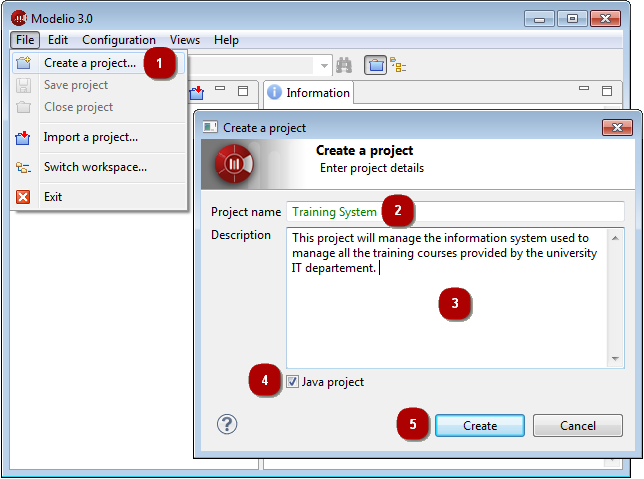
\includegraphics[width=0.8\textwidth]{./figures/modelio-createnewproject.png}
\caption{Creating a new Modelio project.}
\label{figure:modelio-project-creation}
\end{figure}
%
%
%
\begin{enumerate}
\item Launch Modelio.
\item Click on \emph{File} $\rightarrow$ \emph{Create a project...}.
\item Enter the name of the project.
\item Enter the description of the project.
\item If it is envisaged that the project will be connected to a Java development workflow in the future (unrelated to INTO-CPS), you can choose to include the Java Designer module by selecting \emph{Java Project}, otherwise de-select this option.
\item Click on \emph{Create} to create and open the project.
\end{enumerate}
%
%
%
Once you have successfully created a Modelio project, you have to install the Modelio extensions required for INTO-CPS modelling, \emph{i.\@e.\@} both Modelio SysML and INTO-CPS extensions, as described at
%
%
%
\begin{quote}
\url{http://into-cps-association.github.io}
\end{quote}
%
%
%
If both modules have been correctly installed, you should be able to create, under any package, an INTO-CPS Architecture Structure Diagram in order to model the first subsystem of your multi-model.
%
For that, in the Modelio model browser, right click on a \textit{Package} element then in the \textit{INTO-CPS} entry, choose \textit{Architecture Structure Diagram} as shown in \autoref{figure:sysml-create-architecturediagram}.
%
\begin{figure}[hpt!]
\centering
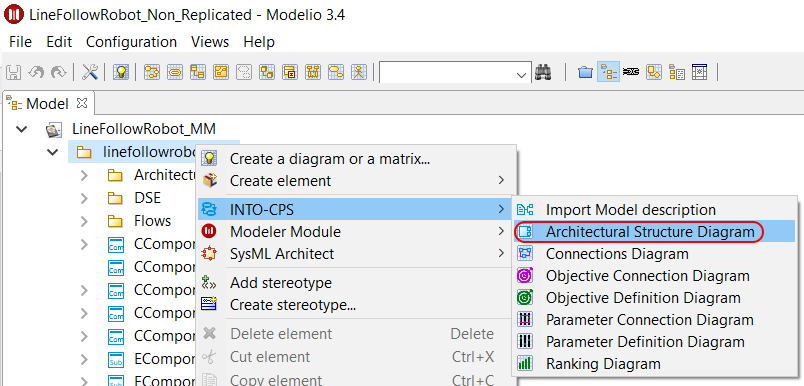
\includegraphics[width=\textwidth]{./figures/sysml-create-architecturediagram.png}
\caption{Creating an Architecture Structure diagram.}
\label{figure:sysml-create-architecturediagram}
\end{figure}
%
Once you are sure that the modules have been correctly installed. You are able to start your INTO-CPS SysML modelling. 
%INTO-CPS Modelling consists in two possible kind of modelling.
%\begin{enumerate}
%  \item In Modelio, right-click on the model block in the tree.
%  \item Select \textit{INTO-CPS} $\rightarrow$ \textit{Generate Model Description} (see \autoref{figure:modelio_export_modelDescription}).
%\end{enumerate}
 
\subsection{INTO-CPS SysML modelling}

INTO-CPS SysML modelling activitIES can be succinctly described as the creation and population of INTO-CPS SysML diagrams.
\autoref{figure:sysml-create-architecturediagram} shows you how to create an Architecture Structure Diagram. 
\autoref{figure:sysml-architecture-diagram} represents an example of an Architecture Structure Diagram.
%
\begin{figure}[hpt!]
\centering
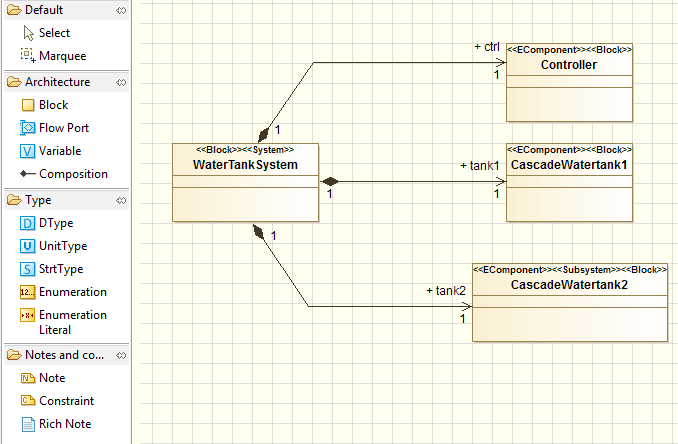
\includegraphics[width=\textwidth]{./figures/sysml-architecture-diagram.png}
\caption{Example Architecture Structure diagram.}
\label{figure:sysml-architecture-diagram}
\end{figure}
%
Besides creating an Architecture Structure Diagram from scratch and specifying by hand the \emph{blocks} of your system, the INTO-CPS extension allows the user to create a block from an existing \texttt{model\allowbreak{}Description\allowbreak{}.xml} file .
%
A \texttt{model\allowbreak{}Description\allowbreak{}.xml} file is an artifact defined in the FMI standard which specifies, in XML format, the public interface of an FMU.
%
To import a \texttt{model\allowbreak{}Description\allowbreak{}.xml} file,
%
%
\begin{enumerate}
\item  Right click in the Modelio model browser on a \textit{Package} element, then in the \textit{INTO-CPS} entry choose \textit{Import Model description}, as shown in \autoref{figure:sysml-reverse}.   
%
\item  Select the desired \texttt{model\allowbreak{}Description\allowbreak{}.xml} file (or the \texttt{.fmu} file that should contain a \texttt{model\allowbreak{}Description\allowbreak{}.xml} file ) in your installation and click on \textit{Import} (\autoref{figure:sysml-reverse-selection}).
\end{enumerate}
%
%
\begin{figure}[hpt!]
\centering
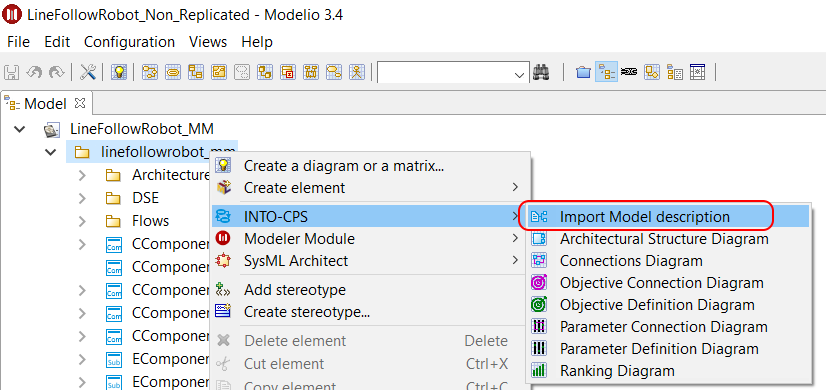
\includegraphics[width=\textwidth]{./figures/sysml-reverse.png}
\caption{Importing an existing model description.}
\label{figure:sysml-reverse}
\end{figure}
%
%
\begin{figure}[hpt!]
\centering
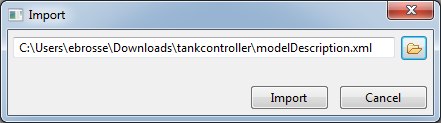
\includegraphics[width=0.7\textwidth]{./figures/sysml-reverse-selection.png}
\caption{Model description selection.}
\label{figure:sysml-reverse-selection}
\end{figure}
%
%
%
This import command creates an Architecture Structure Diagram describing the interface of an INTO-CPS block corresponding to the \texttt{model\allowbreak{}Des\-crip\-tion\allowbreak{}.xml} file imported, \emph{cf.\@} \autoref{figure:sysml-reverse-result}.  
%
%
%
\begin{figure}[hpt!]
\centering
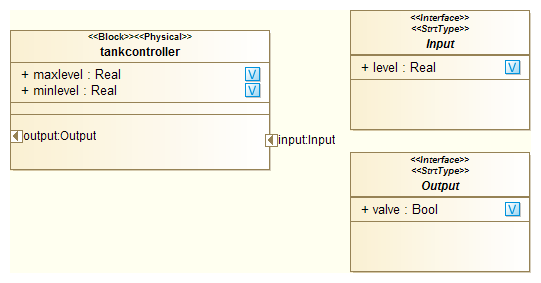
\includegraphics[width=0.8\textwidth]{./figures/sysml-reverse-result.png}
\caption{Result of model description import.}
\label{figure:sysml-reverse-result}
\end{figure}
%
%
%
Once you have created several such blocks, either from scratch or by importing \texttt{model\allowbreak{}Description\allowbreak{}.xml} files, you must eventually connect instances of them in an INTO-CPS Connection Diagram.
%
To create an INTO-CPS Connection diagram, as for an INTO-CPS Architecture Structure Diagram, right click on a \textit{Package} element, then in the \textit{INTO-CPS} entry choose \textit{Connection Diagram}, as shown in \autoref{figure:sysml-create-connectiondiagram}.
%
\autoref{figure:sysml-connectiondiagram-usage} shows the result of creating such a diagram.
%
%
%
\begin{figure}[hpt!]
\centering
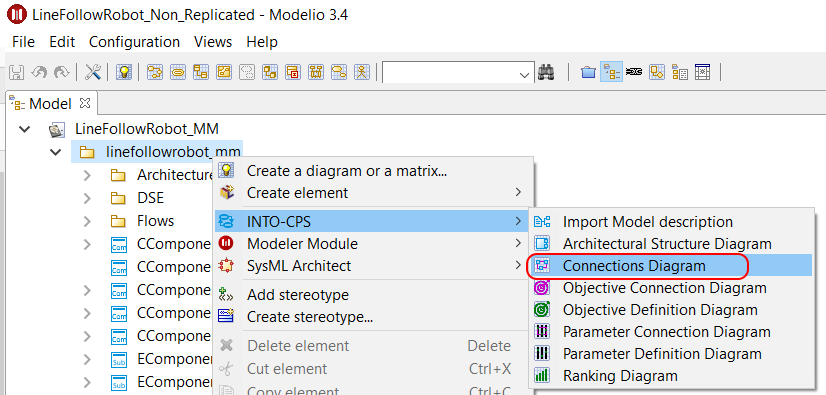
\includegraphics[width=\textwidth]{./figures/sysml-create-connectiondiagram.png}
\caption{Creating a Connection diagram.}
\label{figure:sysml-create-connectiondiagram}
\end{figure}
%
%
%
Once you have created all desired block instances and their ports by using the dedicated command in the Connection Diagram palette, you will be able to model their connections by using the connector creation command (\autoref{figure:sysml-connection-final}).
%
%
%
\begin{figure}[hpt!]
\centering
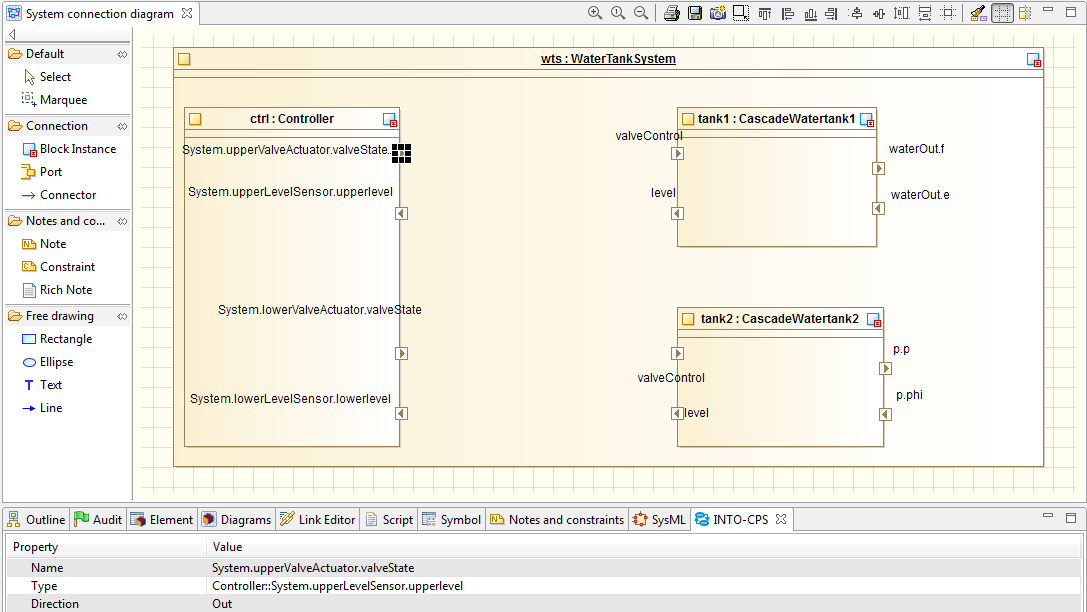
\includegraphics[width=\textwidth]{./figures/sysml-connectiondiagram-usage.png}
\caption{Unpopulated Connection diagram.}
\label{figure:sysml-connectiondiagram-usage}
\end{figure}
%
%
%
\begin{figure}[hpt!]
\centering
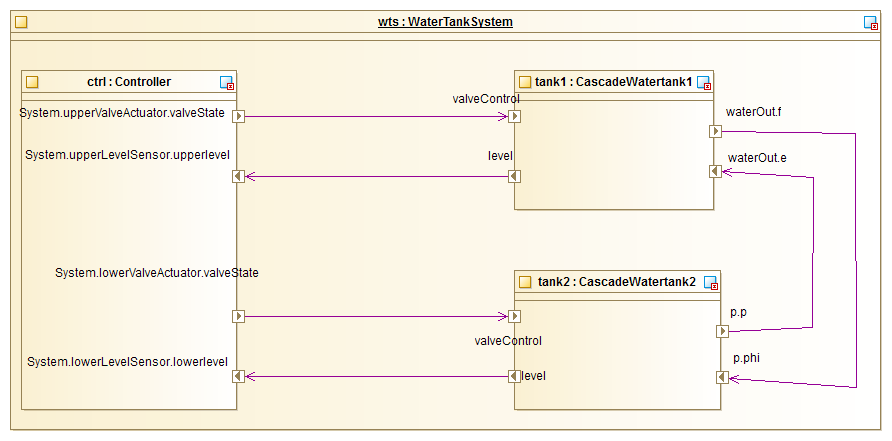
\includegraphics[width=\textwidth]{./figures/sysml-connection-final.png}
\caption{Populated Connection diagram.}
\label{figure:sysml-connection-final}
\end{figure}
%
%
%
At this point your blocks have been defined and the connections have been set.
%
The next step is to simulate your multi-model using the INTO-CPS Application.
%
For that you must first generate a configuration file from your Connection diagram.
%
Select the top element in the desired Connection diagram, right click on it and in the \emph{INTO-CPS} entry choose \emph{Generate configuration}, as shown in \autoref{figure:sysml-generateconfig}.
%
%
%
\begin{figure}[hpt!]
\centering
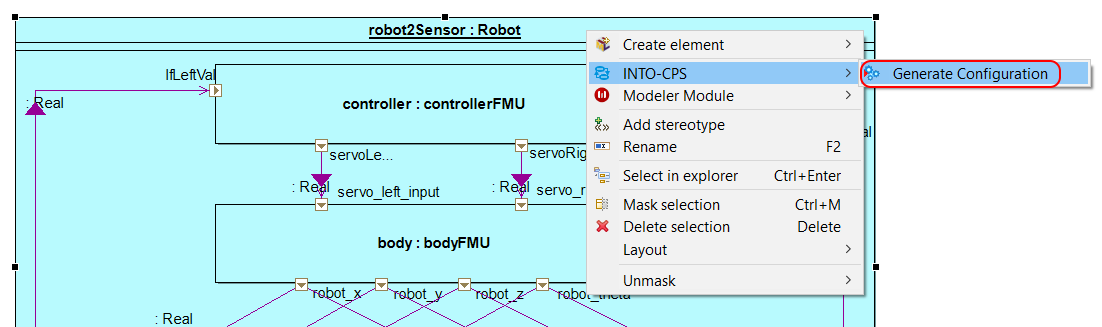
\includegraphics[width=\textwidth]{./figures/sysml-generateconfig.png}
\caption{Generating a configuration file.}
\label{figure:sysml-generateconfig}
\end{figure}
%
%
%
In the final step, choose a relevant name and click on \textit{Generate}.

%\subsection{Exporting \texttt{modelDescription.xml} Files}\label{ch:modelio:sec:export_modeldescription}
The SysML Connection diagram defines the components of the system and their connections.
The internals of these block instances are created in the various modeling tools and exported as FMUs.
The modeling tools Overture, {20-sim} and OpenModelica support importing the interface definition (ports) of the blocks in the Connection diagram by importing a \texttt{modelDescription.xml} file containing the block name and its interface definition.

Follow these steps to export a \texttt{modelDescription.xml} file from Modelio:
%
%
\begin{enumerate}
  \item In Modelio, right-click on the model block in the tree.
  \item Select \textit{INTO-CPS} $\rightarrow$ \textit{Generate Model Description} (see \autoref{figure:modelio_export_modelDescription}).
  \item Choose a file name containing the text ``modelDescription.xml'' and click \textit{Export} (see \autoref{figure:modelio_export_modelDescription_choose_filename}).
\end{enumerate}
%
%
%
\begin{figure}[hpt!]
	\centerline{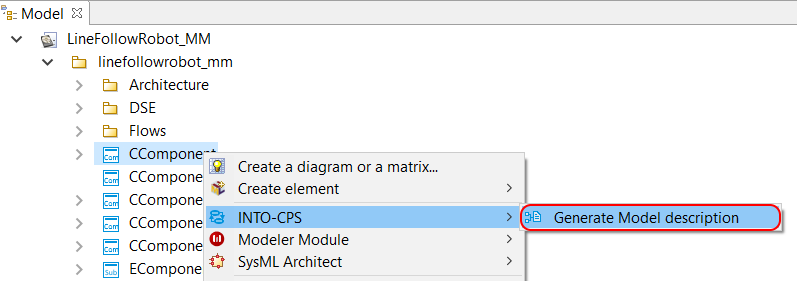
\includegraphics[width=0.9\textwidth]{figures/modelio_export_modelDescription.png}}
	\caption{Exporting a \texttt{modelDescription.xml} file.}
	\label{figure:modelio_export_modelDescription}
\end{figure}
%
%
%
\begin{figure}[hpt!]
	\centerline{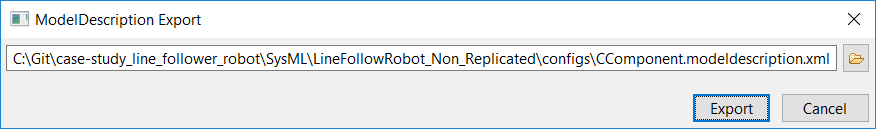
\includegraphics[width=0.8\textwidth]{figures/modelio_export_modelDescription_choose_filename.png}}
	\caption{Naming the model description file.}
	\label{figure:modelio_export_modelDescription_choose_filename}
\end{figure}

\subsection{DSE Modelling}

For design space exploration (DSE) purposes, a DSE model can be constructed in Modelio as well. This modelling is done by specifying mainly a DSE analysis, its parameters, its objectives and a ranking method. 
\autoref{figure:modelio_dse_objective_definition} depicts an example of a DSE objective definition.
%
\begin{figure}[hpt!]
	\centerline{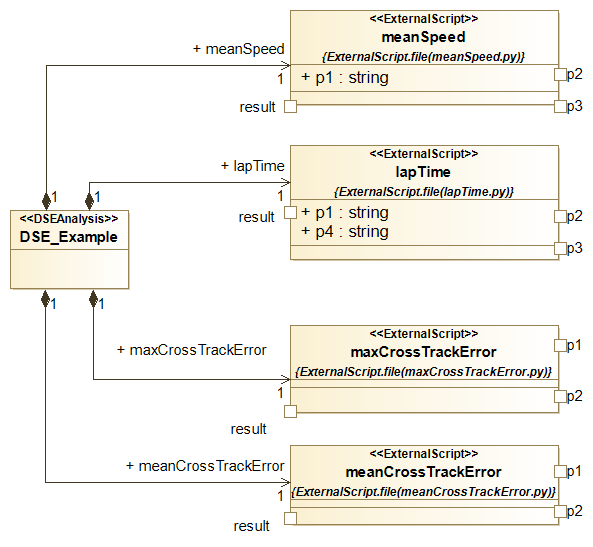
\includegraphics[width=0.5\textwidth]{figures/modelio/dse_objective_definition.png}}
	\caption{DSE Objective definition.}
	\label{figure:modelio_dse_objective_definition}
\end{figure}
%
More details and examples can be found in Deliverable D4.2c \cite{INTOCPSD4.2c}.

Once the DSE model has been created, the DSE analysis can be exported to the INTO-CPS Application. To do so, right-click on \emph{DSE Analysis} in the model tree as depicted in \autoref{figure:modelio_dse_export_command}.   
%
\begin{figure}[hpt!]
	\centerline{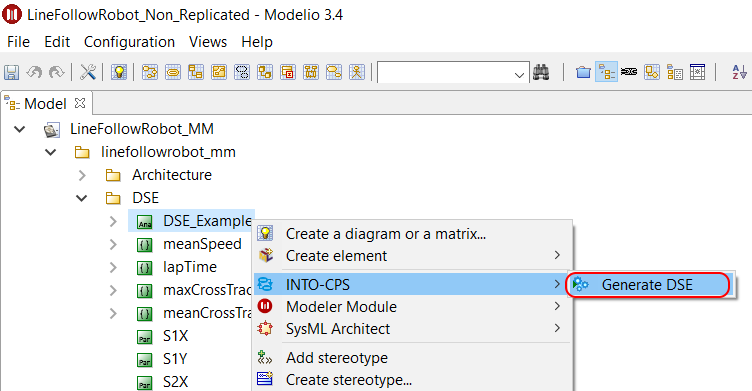
\includegraphics[width=0.8\textwidth]{figures/modelio/dse_export_command.png}}
	\caption{DSE Export command.}
	\label{figure:modelio_dse_export_command}
\end{figure}
%
In the final step, choose a relevant name and click on \textit{Export}.
%
%
%
\subsection{Behavioural Modelling}\label{sec:SysML:BehaviouralModelling}
For test generation and/or model-checking analysis, a behavioural model of the system is required. This is usually referred to as {\em test model} in order to indicate its purpose. It is typically not identical to the design model, because it can omit or abstract implementation details.
%
The test model needs to capture all inputs and outputs and describe the system's reactions to inputs by means of one or more deterministic state machine diagram. Timing behaviour should be included by means of timers and timer-guarded transitions.
%
For more details and examples refer to the RTT-MBT Manual~\cite{VSI-mbt-man}.

Once the behavioural model has been specified, the \emph{entire model} must be exported in XMI format. To do so, right-click on the \emph{top package} in the model tree as depicted in \autoref{figure:modelio_xmi_export_command}.   
%
\begin{figure}[hpt!]
	\centerline{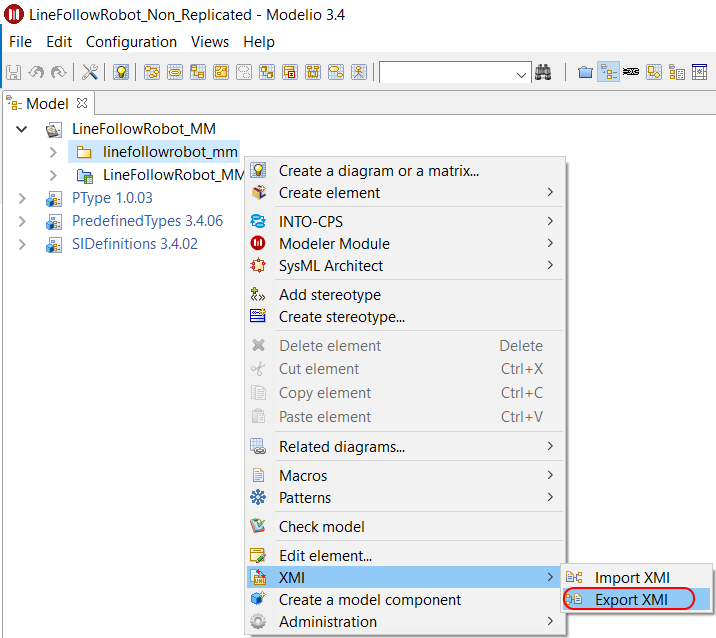
\includegraphics[width=0.8\textwidth]{figures/modelio/xmi_export_command.png}}
	\caption{XMI Export command.}
	\label{figure:modelio_xmi_export_command}
\end{figure}
%
Then select the file path by using the XMI export window, as shown in \autoref{figure:modelio_xmi_export_window}. Note that compatibility must be set to "EMG UML 3.0.0" and the file extension to ".xmi".
%
\begin{figure}[hpt!]
	\centerline{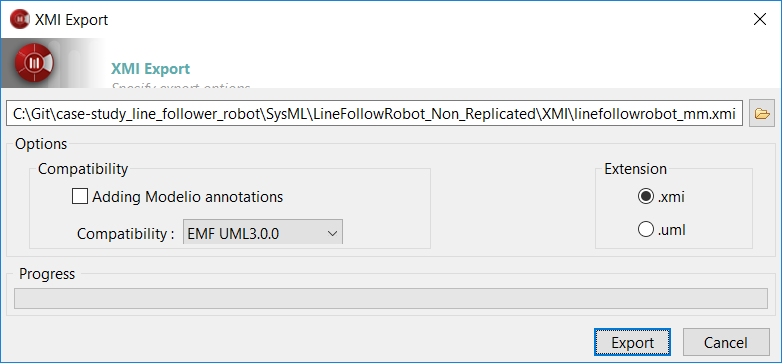
\includegraphics[width=0.7\textwidth]{figures/modelio/xmi_export_window.png}}
	\caption{XMI export windows.}
	\label{figure:modelio_xmi_export_window}
\end{figure}


\clearpage